% Made up for the tikra benchmark.
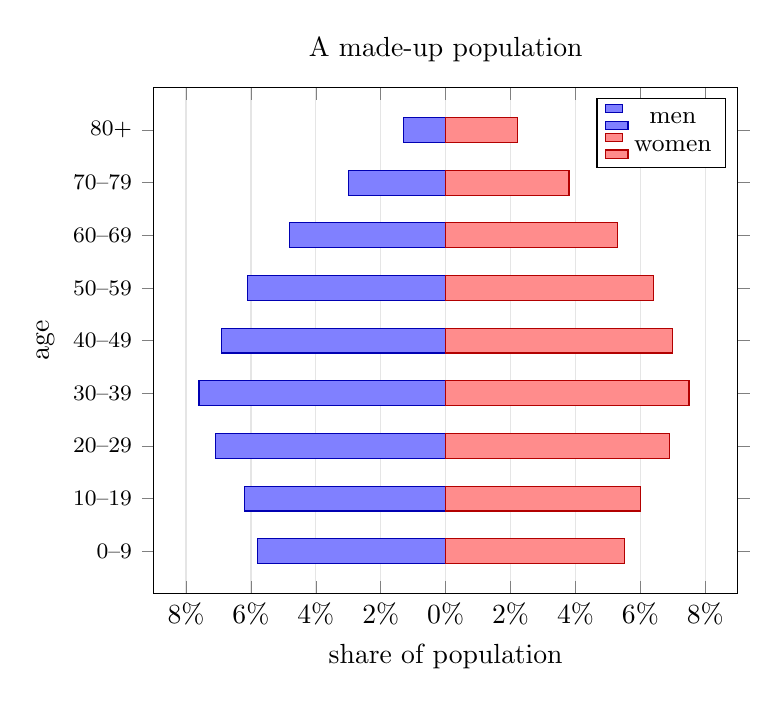
\begin{tikzpicture}
\begin{axis}[xbar, bar shift=0pt, bar width=9pt, width=9cm, height=8cm, xmin=-9, xmax=9,
    ytick={0,...,8}, yticklabels={0--9, 10--19, 20--29, 30--39, 40--49, 50--59, 60--69, 70--79, 80+},
    xtick={-8,-6,...,8}, xticklabels={8\%,6\%,4\%,2\%,0\%,2\%,4\%,6\%,8\%},
    xlabel={share of population}, ylabel={age}, title={A made-up population},
    y tick label style={font=\footnotesize},
    legend style={at={(0.98,0.98)}, anchor=north east, font=\small}, xmajorgrids, grid style={gray!20}]
  \addplot[fill=blue!50, draw=blue!70!black] coordinates
    {(-5.8,0) (-6.2,1) (-7.1,2) (-7.6,3) (-6.9,4) (-6.1,5) (-4.8,6) (-3.0,7) (-1.3,8)};
  \addplot[fill=red!45, draw=red!70!black] coordinates
    {(5.5,0) (6.0,1) (6.9,2) (7.5,3) (7.0,4) (6.4,5) (5.3,6) (3.8,7) (2.2,8)};
  \legend{men, women}
\end{axis}
\end{tikzpicture}
